\documentclass[thesis.tex]{subfiles}

\begin{document}

\chapter{KdV5}

\section{Periodic 2-pulse}

In this section, we will consider the simplest case, which is the periodic 2-pulse. Let $Q_2(x)$ be a periodic 2-pulse constructed as in Theorem \ref{perexist} with scaling parameter $r$, baseline length parameters $\{b_0^0, b_1^0 \}$ with $b_j^0 = \exp\left(-\frac{m_j \pi}{\rho}\right)$, and phase parameter $\theta$. Without loss of generality, take $m_0 \in \{0, 1\}$. Let $b_0(r)$ and $b_1(r)$ be the associated length parameters, and let $X_0$ and $X_1$ be the actual pulse distances, whose dependence on these parameters is given in Theorem \ref{perexist}. Finally, let $X = X_0 + X_1$.  

By Theorem \ref{blockmatrixtheorem}, the eigenvalues for the linearization about $Q_2(x)$ can be found by finding the zeros of the determinant of a block matrix. To leading order, this is block diagonal, thus we expect to find the interaction eigenvalues when $A - \lambda^2 M I$ is singular and the essential spectrum eigenvalues when $K(\lambda)$ is singular. We anticipate the following eigenvalue pattern.
\begin{itemize}
\item There will be a pair of nonzero interaction eigenvalues at $\lambda = \pm \sqrt{-2a(r)/M}$, where 
\[
a(r) = a_0(r) + a_1(r) = \langle \Psi(X_0), Q'(-X_0) \rangle + \langle \Psi(X_1), Q'(-X_1) \rangle = \mathcal{O}(r)
\]
and the $a_j(r)$ are defined in Theorem \ref{blockmatrixtheorem}. We have made the dependence on $r$ explicit.
\item There will be essential spectrum eigenvalues at
\[
\lambda = \pm c \frac{k \pi i}{X}
\]
for integer $k$, where $X = \mathcal{O}(|\log r|)$.
\end{itemize}

We are interested in two parameter regimes. First, we will consider the case where $r$ is sufficiently small so the interaction eigenvalues are smaller in magnitude than the nonzero essential spectrum eigenvalues. Next, we will consider the case when a purely imaginary interaction eigenvalue is close to the first nonzero essential spectrum eigenvalue, in which case we will have an instability bubble.

\subsection{Case 1: essential spectrum is out of the way}\label{section:2pernobubble}

In this section, we consider the case where the essential spectrum is ``out of the way'' of any interaction eigenvalues. 

Let $a(r) = a_0(r) + a_1(r)$, where the $a_j(r)$ are defined in Theorem \ref{blockmatrixtheorem}. Since $a(r) = \mathcal{O}(r)$, let $a(r) = r \tilde{a}(r)$. In the next theorem we prove that if $\tilde{a}(0) \neq 0$, the only possible eigenvalue patterns are those shown in \cref{fig:2ppatterns}. First we show that the degenerate case $\tilde{a}(0) = 0$ only occurs at the pitchfork bifurcation points.

\begin{lemma}
$\tilde{a}(0) = 0$ if and only if the 2-pulse $Q_2(x)$ is parameterized by $b_0(0) = b_1(0) = p_k^*$ for $k \in \{0, 1\}$, where $p_k^*$ is one of the pitchfork bifurcation points.
\begin{proof}
Numerics strongly suggests this is true. We can prove it along the diagonal, in a neighborhood of the pitchfork points, and sufficiently far from the diagonal.
\end{proof}
\end{lemma}

We can now state the main theorem of the section, which locates the eigenvalues of the linearization of the PDE \cref{genPDE} about $Q_2(x)$.

\begin{theorem}\label{theorem:2peigscase1}
Assume Hypotheses \ref{Ehyp}, \ref{Hhyp}, \ref{hypeqhyp}, \ref{Qexistshyp}, \ref{H0transversehyp}, \ref{Melnikov2hyp}, and \ref{Adistincteigs}. Choose baseline length parameters
\[
b_0^0 = \exp\left(-\frac{m_0 \pi}{\rho}\right), \quad b_1^0 = \exp\left(-\frac{m_1 \pi}{\rho}\right),
\] 
with $m_0 \in \{ 0, 1\}$ and phase parameter $\theta$. Let $Q_2(x; r)$ be the family of periodic 2-pulse solutions corresponding to our choice of parameters, where $r \in \mathcal{R}$ with $r \leq r_*$. Let $\{ b_0(r), b_1(r) \}$ be the length parameters associated with $Q_2(x; r)$.

Let $\delta > 0$ and $M$ be as in Theorem \ref{blockmatrixtheorem}. Let $a_0(r)$, and $a_1(r)$ be the coefficients of the matrix $A$ in \ref{blockmatrixtheorem}, where we have made the dependence on $r$ explicit. Let $a(r) = a_0(r) + a_1(r)$, and take $a(r) = r \tilde{a}(r)$. Choose $r_0$ sufficiently small so that 
\begin{equation}\label{nobubblecond}
\left| \sqrt{\frac{2 \tilde{a}(0)}{M}}\right|r_0^{1/2} \leq \frac{1}{2} \frac{c}{\left( 2 |\log r_0| + |\log( b_0(0) b_1(0) |\right)}
\end{equation}
Then the following are true.

\begin{enumerate}[(i)]
\item Choose any positive integer $N$ such that
\[
\frac{N c \pi}{2 |\log r_0| + |\log b_0(0) b_1(0)| } < \delta
\]
Then there exists $r_1 \leq r_0$ such that for all $r\leq r_1$, there are $2N$ nonzero essential spectrum eigenvalues $\lambda = \{ \pm \lambda_m^{\text{ess}} : m = 1, \dots, N\}$, where
\[
\lambda_m^{\text{ess}}(r) = c \frac{m \pi i}{X}+  \mathcal{O}\left( \frac{1}{|\log r|^2} \right)
\]
is on the imaginary axis and $X = \mathcal{O}(|\log r|)$

\item If $\tilde{a}(0) \neq 0$, then the following are true.
\begin{enumerate}
	\item There exists $r_2 \leq r_0$ such that for all $r \leq r_2$, there is an eigenvalue at 0 with algebraic multiplicity 3.

	\item There exists $r_3 \leq r_0$ such that for all $r \leq r_3$, there is a pair of interaction eigenvalues located at
	\begin{align*}
	\lambda^{\text{int}} = \pm \left( \sqrt{-\frac{2 \tilde{a}(r)}{M}}r^{1/2} + \mathcal{O}\left( r \right) \right)
	\end{align*}
	If $M > 0$, then NUMERICS STRONGLY SUGGESTS THAT these are real if $m_0 = 0$ and purely imaginary if $m_0 = 1$. (This is reversed if $M < 0)$. 
\end{enumerate}
\item DEGENERATE CASE HERE. This is the eigenvalue bifurcations at the pitchfork points on the diagonal.

\end{enumerate}
\end{theorem}

\begin{remark}
In terms of the physical parameters, the condition \cref{nobubblecond} is equivalent to  
\[
\left| \sqrt{\frac{2a(r_0)}{M}} \right| \leq \frac{c}{2 X}
\]
\end{remark}

\subsection{Case 2: instability bubble}\label{section:2perbubble}

In this section, we consider what happens when a purely imaginary interaction eigenvalues is close to an essential spectrum eigenvalue. We will show that under certain conditions, an instability bubble forms when essential spectrum eigenvalues (positive Krein signature) collide with interaction eigenvalues (negative Krein signature) on the imaginary axis. For this to happen, we require $2a/M > 0$, so that there is an imaginary interaction eigenvalue in play.

For an instability bubble to occur, an essential spectrum eigenvalue must get close to an interaction eigenvalue. Since the two interaction eigenvalues are $\mathcal{O}(r^{1/2})$ and the smallest nonzero essential spectrum eigenvalues is $\mathcal{O}(|\log r|)$, if we decrease $r$, this can never occur. Thus the only way to achieve this is to keep $r$ fixed, so that that the pulse distance $X_0$ is constant to leading order, and to increase $X_1$.

Before we state the theorem, we will illustrate what occurs graphically. Let $s \in [-2, 2]$ be a dimensionless parameter which measures the distance on the imaginary axis between $\lambda_1 i$ and $\lambda_* i$; $s = 0$ corresponds to $X = X^*$. Let $R = R_0 / \sqrt{X^*}$, where $R_0$ is a parameter that depends the primary pulse and on intrinsic properties of the system. We assume that $R_0 > 0$, which can be verified checked numerically.

We will show that there is a pair of eigenvalues $\lambda_{1,2}$ near $\lambda_* i$ which can be parameterized by $s$. As $s$ decreases from $2$ to $-2$, a pair of purely imaginary eigenvalues collides near $\lambda_* i + i \sqrt{R}$, moves off of the imaginary axis, travels on a circle of radius $\sqrt{R}$ centered at $\lambda_* i$, and recombines near $\lambda_* i - i \sqrt{R}$. This is illustrated in \cref{fig:kreinbubbles}. The numerics match this picture.
\begin{figure}[H]
\begin{center}
\begin{tabular}{ccc}
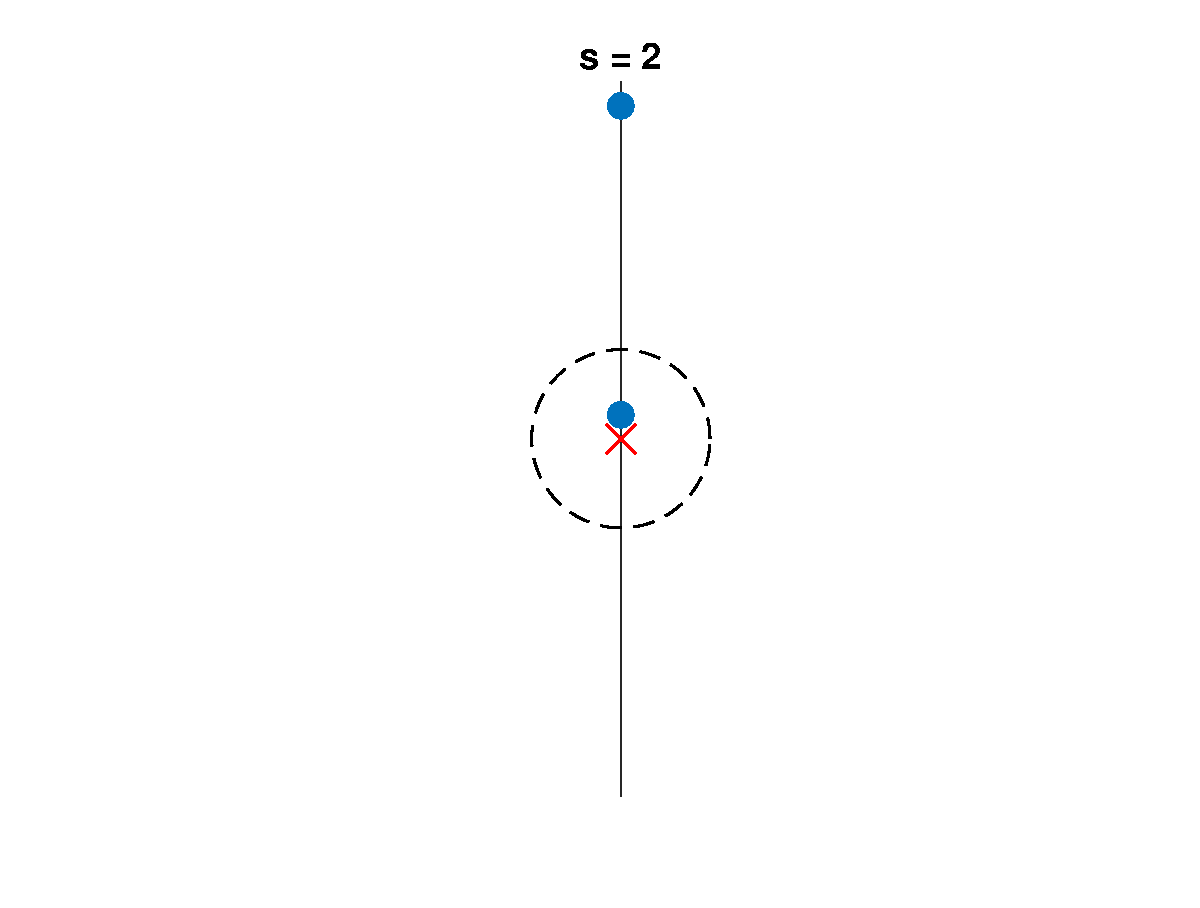
\includegraphics[width=5cm]{images/kreinbubbles/bubble2R} &
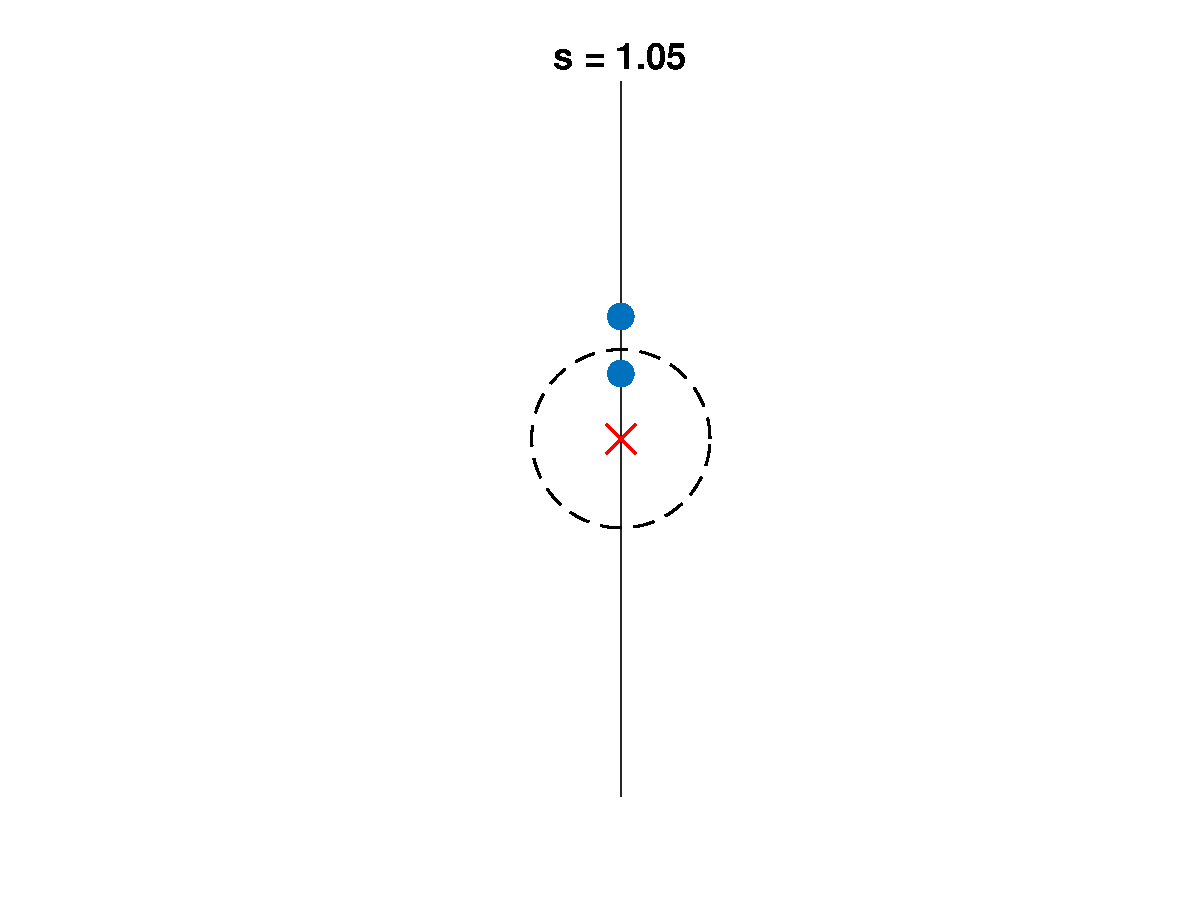
\includegraphics[width=5cm]{images/kreinbubbles/bubble105R} &
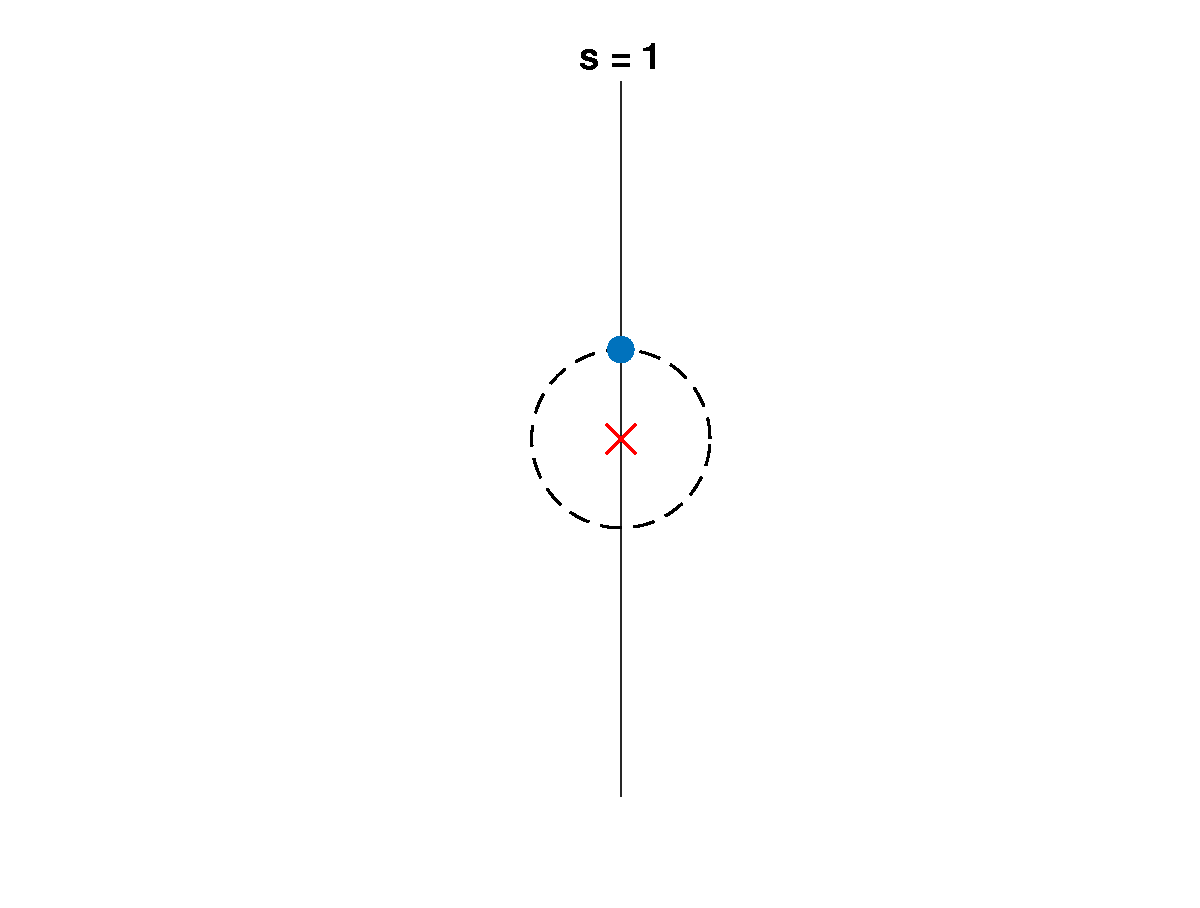
\includegraphics[width=5cm]{images/kreinbubbles/bubbleR} \\
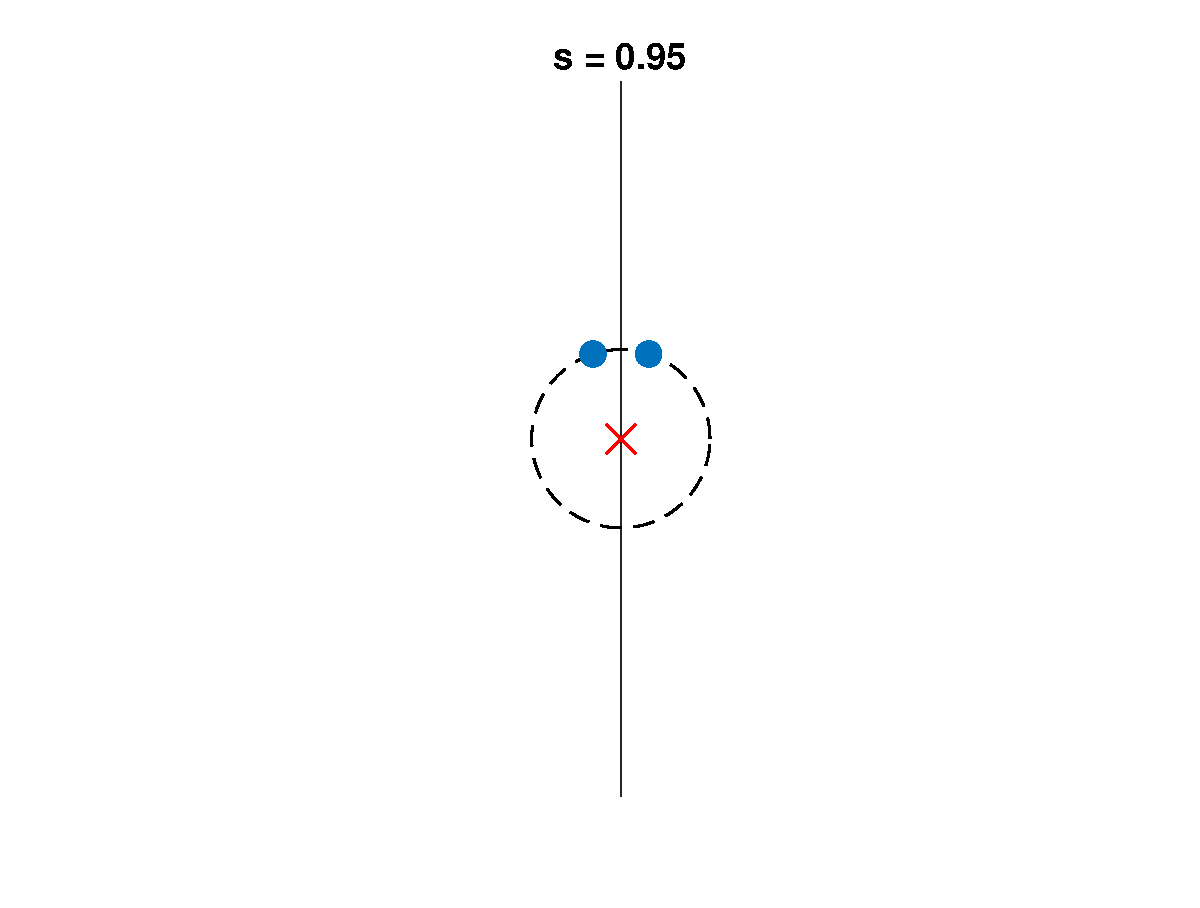
\includegraphics[width=5cm]{images/kreinbubbles/bubble095R} &
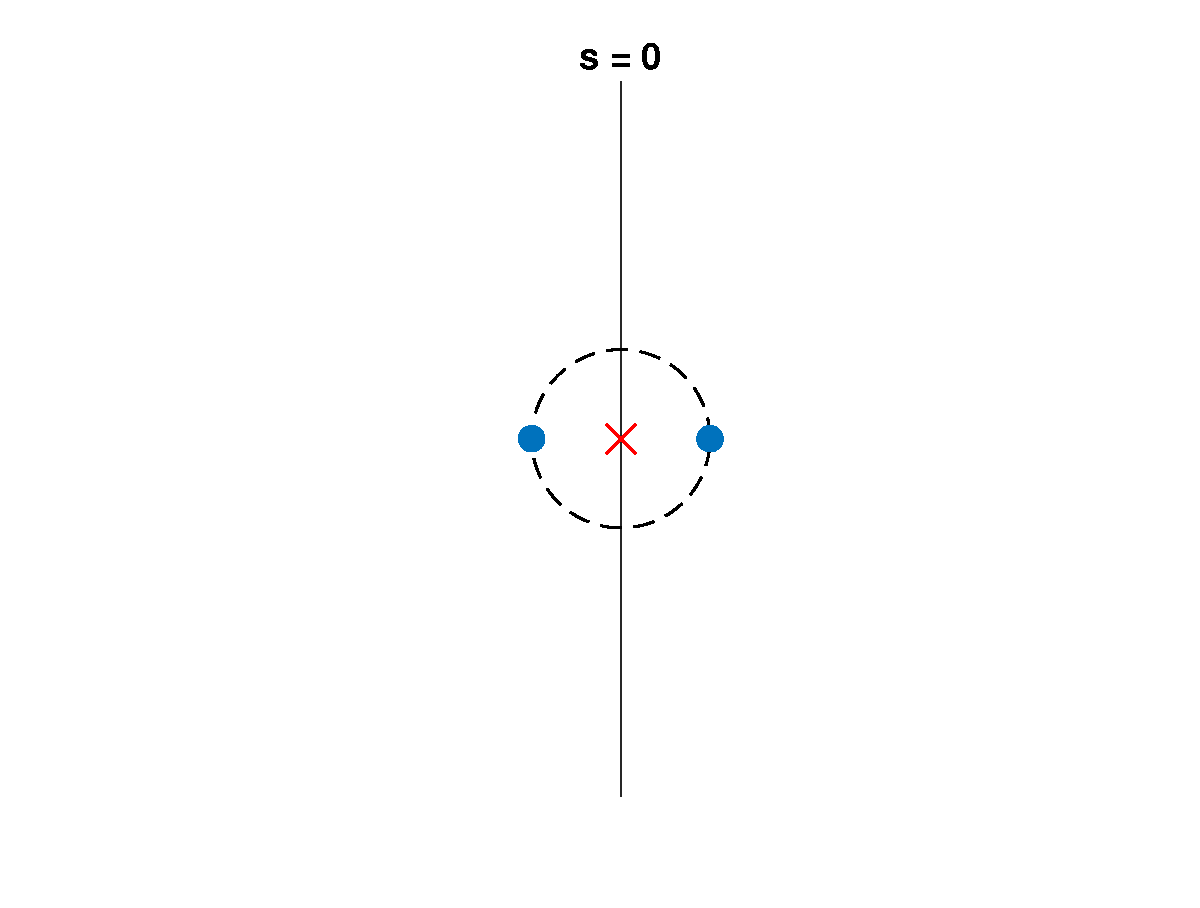
\includegraphics[width=5cm]{images/kreinbubbles/bubble0} &
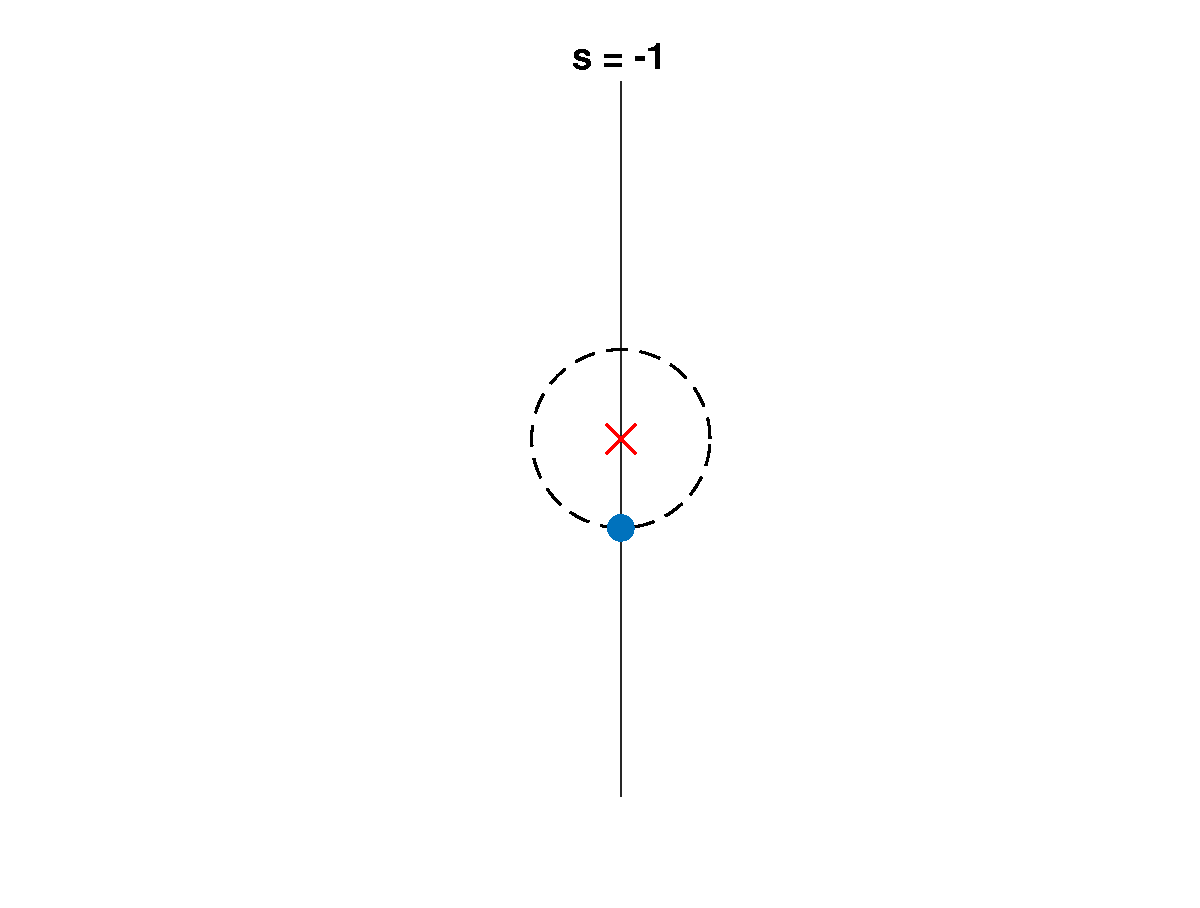
\includegraphics[width=5cm]{images/kreinbubbles/bubbleminusR}
\end{tabular}
\caption{Plot of the complex plane illustrating eigenvalue collision and Krein bubble as parameter $s$ is decreased. Blue dots are the pair of eigenvalues. Red cross is the point $\lambda_* i$. Vertical line is the imaginary axis. Black dotted circle is the circle of radius $\sqrt{R}$ around $\lambda_*$ }
\label{fig:kreinbubbles}
\end{center}
\end{figure}
We will call the instability bubble a Krein bubble, since it results from the collision of two imaginary eigenvalues with opposite Krein signatures. Inside the Krein bubble, the eigenvalues $\lambda_{1,2}$ are symmetric across the imaginary axis. Outside the Krein bubble, there is no such symmetry for $\lambda_{1,2}$; since $\lambda_{1,2}$ are purely imaginary, Hamiltonian symmetry tells that there exist eigenvalues $-\lambda_{1,2}$ which are below the real axis.

In the following theorem, we prove that Krein bubbles occur. For simplicity, we will only consider the first Krein bubble, which occurs when the collision occurs between an imaginary interaction eigenvalue and the first nonzero essential spectrum eigenvalue. Since the bubbles are formed as $X$ is varied near $X^*$, we will parameterize both $X$ and the eigenvalues $\lambda_{1,2}$ by a single dimensionless parameter $s \in [-2, 2]$. 

\begin{theorem}\label{theorem:kreinbubbles}
Assume Hypotheses \ref{Ehyp}, \ref{Hhyp}, \ref{hypeqhyp}, \ref{Qexistshyp}, \ref{H0transversehyp}, \ref{Melnikov2hyp}, and \ref{Adistincteigs}. Choose baseline length parameters
\[
b_0^0 = \exp\left(-\frac{m_0 \pi}{\rho}\right), \quad b_1^0 = \exp\left(-\frac{m_1 \pi}{\rho}\right),
\] 
with $m_0 \in \{ 0, 1\}$ and phase parameter $\theta$. Let $Q_2(x; r)$ be the family of periodic 2-pulse solutions corresponding to our choice of parameters, where $r \in \mathcal{R}$ with $r \leq r_*$. Let $\{ b_0(r), b_1(r) \}$ be the length parameters associated with $Q_2(x; r)$.

Let $\delta > 0$, $M$, and $M^c$ be as in Theorem \ref{blockmatrixtheorem}. Let $a_0(r)$, and $a_1(r)$ be the coefficients of the matrix $A$ in \ref{blockmatrixtheorem}, and let $a(r) = a_0(r) + a_1(r)$. Let
\begin{itemize}
\item $\lambda_1 = c \frac{\pi}{X}$.
\item $\lambda_* = \sqrt{\frac{2 a(r) }{M}}$
\item $X^* = \frac{c \pi}{\lambda_*}$
\item $R_0 = \frac{M^c q(X_0)}{M}$, where $q(x)$ is the first component of the primary pulse $Q(x)$.
\item $R = \lambda_*^2 R_0 \frac{X_0}{X}$
\end{itemize}

Assume $R_0 > 0$. Then there exists $r_1 
leq r_*$ such that for all $r \leq r_1$, the following is true. Let $s \in [-2, 2]$. For $X = X(s)$ close to $X^*$, there exists a pair of eigenvalues located at
\begin{align*}
\lambda_{1,2}(s) = \left( \lambda_* + s \sqrt{R} \right) i \pm \sqrt{R(1 - s^2)} + \text{``h.o.t.''}
\end{align*}
where
\[
X(s) = \frac{c \pi}{s \sqrt{R} + \lambda_*}
\]
and $X(0) = X^*$. These eigenvalues have the following configuration.
\begin{itemize}
\item For $|s| < 1$, $\lambda_{1,2}(s)$ is symmetric across the imaginary axis, i.e. $\lambda_2(s) = -\overline{\lambda_1}(s)$. For $s = 0$, these are given by
\[
\lambda_{1,2}(s) = \lambda_* i \pm (\sqrt{R} + ``h.o.t.'')
\]
\item For $|s| \in (1, 2]$, $\lambda_{1,2}(s)$
are purely imaginary. For $s = 2$, one of $\lambda_{1,2}(s)$ is close to $\lambda_* i$.
\item At $s = \pm 1$, $\lambda_{1,2}(s)$ collide on the imaginary axis at 
\[
\lambda_{1,2}(s) = \lambda_* i \pm (\sqrt{R} + ``h.o.t.'')
\]
\end{itemize}
For $|s| \leq 1$, the eigenvalues $\lambda_{1,2}(s)$ are, to leading order, located on a circle of radius $\sqrt{R}$ about $\lambda_* i$ in the complex plane, where
\[
\sqrt{R} = \mathcal{O}\left( r^{3/4}\frac{X_0}{X} \right)
\]
\end{theorem}

\section{Determinant of block matrix}\label{sec:blockdet}


To find the eigenvalues, we will find the zeros of \cref{2detBeqmu}. We will do this for several specific cases.

\section{Eigenvalues of $A$}

First, we compute the coefficients $a_j(r)$ of the matrix $A$ in lower right block of the block matrix.


Next, we prove a relationship between the sign of $\tilde{a}(0)$ and the geometry of the 2-periodic pulse. We will the be able to characterize the set of length parameters for which $\tilde{a}(0) = 0$.

\begin{lemma}\label{lemma:tildea0char}
Let $Q_2(x)$ be a periodic 2-pulse constructed with baseline length parameters 
\begin{align*}
b_0^0 &= \exp\left(-\frac{m_0 \pi}{\rho}\right) \\
b_1^0 &= \exp\left(-\frac{m_1 \pi}{\rho}\right)
\end{align*}
and phase parameter $\theta$, where $m_0 \in \{0, 1\}$ and $m_1 \geq m_0$. Let $b_0(r)$ and $b_1(r)$ be the length parameters.
\begin{enumerate}
	\item $\tilde{a}(0) = 0$ if and only if the 2-pulse $Q_2(x)$ is parameterized by $b_0(0) = b_1(0) = p_k^*$ for $k \in \{0, 1\}$, where $p_k^*$ is one of the pitchfork bifurcation points.
	\item If this is not the case, then the sign of $\tilde{a}(0)$ depends only on $m_0$. Specifically,
	\begin{enumerate}
		\item If $m_0 = 0$, $\tilde{a}(0) > 0$.
		\item If $m_0 = 1$, $\tilde{a}(0) < 0$.
	\end{enumerate}
\end{enumerate}
\begin{proof}
For convenience, let $b_j = b_j(0)$ and $\tilde{a} = \tilde{a}(0)$. From \cref{lemma:ajparam}, scaling out a factor of $r$, we have
\begin{align*}
\tilde{a}(0) &= s_0 e^{\alpha_0 \phi/\beta_0}\left[ b_0 ( \beta_0 \cos(-\rho \log b_0 ) - \alpha_0 \sin (-\rho \log b_0 ))  + b_1 ( \beta_0 \cos(-\rho \log b_1 ) - \alpha_0 \sin (-\rho \log b_1 )) \right]
\end{align*}
Factoring out $\alpha_0$, this becomes
\begin{equation}\label{tildea0}
\tilde{a}(0) = s_0 e^{\alpha_0 \phi/\beta_0} \alpha_0 \left[ b_0 ( \rho \cos(-\rho \log b_0 ) - \sin (-\rho \log b_0 ))  + b_1 ( \rho \cos(-\rho \log b_1 ) - \sin (-\rho \log b_1 )) \right]
\end{equation}

We take the parameterization from Lemma \ref{thetaparamlemma}. We will consider two cases.

\begin{enumerate}
\item Symmetric periodic 2-pulse, i.e. $m_0 = m_1 = m$. When $r = 0$, from Lemma \ref{thetaparamlemma}, we have the parameterization
\begin{equation*}
\begin{aligned}
b_1^*(\theta) &= e^{-\frac{1}{\rho}(m \pi - \theta) } \\
b_0^*(\theta) &= e^{-\frac{1}{\rho}(m \pi - \theta) }
\end{aligned}
\end{equation*}
Substituting these into \cref{tildea0}, 
\begin{align*}
\tilde{a}(0) &= 2 s_0 \alpha_0 e^{\alpha_0 \phi/\beta_0} e^{-\frac{1}{\rho}(m \pi + \theta) } \left( \rho \cos(m \pi + \theta) - \sin (m \pi + \theta) \right) \\
&= 2 (-1)^m s_0 \alpha_0 e^{\alpha_0 \phi/\beta_0} e^{-\frac{1}{\rho}(m \pi - \theta) } \left( \rho \cos\theta - \sin\theta \right) \\
\end{align*}
This is 0 if and only if $\rho \cos\theta - \sin\theta = 0$. From Lemma \ref{pitchforkH}, this is true if and only if $\theta = p^*_k$, where $p^*_k$ is one of the pitchfork bifurcation points. In terms of $\theta \in I\rho = [-\pi+\arctan \rho, \arctan \rho]$, this only occurs when $\theta$ is one of the endpoints of $I_\rho$. Since $\rho \cos\theta + \sin\theta \geq 0$ for $\theta \in I_\rho$, the sign of $\tilde{a}(0)$ away from the pitchfork bifurcation points is independent of $\theta$ and depends only on the integer $m$. Thus for $m = 0$, $\tilde{a}(0) > 0$ and for $m = 1$, $\tilde{a}(0) < 0$.

\item Asymmetric periodic 2-pulse with $m_1 + m_0 + m$, with $m \geq 1$. From Lemma \ref{thetaparamlemma}, we have the parameterization
\begin{equation*}
\begin{aligned}
b_1^*(\theta) &= e^{-\frac{1}{\rho}((m_0 + m) \pi - \theta) } \\
b_0^*(\theta) &= e^{-\frac{1}{\rho}(m_0 \pi - \theta^*(\theta, m)) } \\
\end{aligned}
\end{equation*}
where we recall from Lemma \ref{thetaparamlemma} that $\theta^*$ only depends on the difference $m_1 - m_0$. In this case, we have
\begin{align*}
\tilde{a}(0) &= s_0 e^{\alpha_0 \phi/\beta_0} \alpha_0 \Big[ (-1)^{m_0} e^{-\frac{1}{\rho}(m_0 \pi - \theta^*(\theta, m))} \left( \rho \cos(\theta^*(\theta, m)) + \sin(\theta^*(\theta, m)) \right) \\
&\qquad + (-1)^{m_0 + m} e^{-\frac{1}{\rho}((m_0 + m) \pi - \theta) } ( \rho \cos(\theta) + \sin (\theta)) \Big] \\
&= (-1)^{m_0} s_0 \alpha_0 e^{\alpha_0 \phi/\beta_0} e^{-\frac{1}{\rho} m_0 \pi} \Big[ e^{\frac{1}{\rho} \theta^*(\theta, m)} \left( \rho \cos(\theta^*(\theta, m)) + \sin(\theta^*(\theta, m)) \right) \\
&\qquad + (-1)^{m} e^{-\frac{1}{\rho}(m \pi - \theta) } ( \rho \cos(\theta) + \sin (\theta)) \Big]
\end{align*}
From Lemma \ref{thetaparamlemma}, if $m = 1$ and $\theta = \pi - \arctan \rho$, we are at one of the pitchfork bifurcation points; it is not hard to show that using this parameterization we will also have $\tilde{a}(0) = 0$. For any other $m$ and $\theta$, recall from part (4c) of the proof of Lemma \ref{thetaparamlemma} that $|\theta^*(\theta, m)| < |\theta|$. 
THIS IS STILL INCOMPLETE. THE COMPUTATIONS ARE TEDIOUS.
\end{enumerate}
\end{proof}
\end{lemma}



\subsection{Degenerate case}

The final case to consider is when $\tilde{a}(0) \neq 0$, which occurs only at the two pitchfork bifurcation points. Starting with \cref{2detBint4}, since we know there are always two eigenvalues at 0 corresponding to $\partial_x Q_2(x)$ and $\partial_c Q_2(x)$. By \cref{lemma:centereigenfn}, there is a third eigenvalue at 0 corresponding to eigenfunction $V_n^c(x)$. Thus we can divide by $\tilde{\mu}^3$ to get
\begin{equation}\label{2degen1}
\begin{aligned}
G(\tilde{\mu},r) = (\tilde{\mu} - \tilde{\mu}_*(r))(\tilde{\mu} + \tilde{\mu}_*(r)) + \mathcal{O}\left( r |\log r|^2 + r^{1/2} \right)
\end{aligned}
\end{equation}
where we used $X = \mathcal{O}(|\log r|)$. When $r = 0$, this becomes
\[
G(\tilde{\mu},0) = (\tilde{\mu} - \tilde{\mu}_*(0))(\tilde{\mu} + \tilde{\mu}_*(0))
\]
We are interested in the case when $\tilde{\mu}$ is close to 0, which occurs when $\tilde{a}(0)$ is close to 0. Substituting $\mu_*(0) = \sqrt{2 \tilde{a}(0)/M c^2}$, this becomes
\begin{equation*}
G(\tilde{\mu},0) = \left( \tilde{\mu} - \sqrt{\frac{2 \tilde{a}(0)}{M c^2}} \right)\left(\tilde{\mu} +  \sqrt{\frac{2 \tilde{a}(0)}{M c^2}} \right) \\
= \tilde{\mu}^2 - \frac{2}{M c^2}\tilde{a}(0)
\end{equation*}
Since $\tilde{a}(0) = 0$ only at the two pitchfork bifurcations, we will look at one of them. The other one will be similar. 

Take the case $m_0 = m_1 = 0$. As $\theta$ is varied in a small neighborhood of $\theta = -\arctan \rho$,
\begin{align*}
\tilde{a}(0) &> 0 && \theta < -\arctan \rho \\
\tilde{a}(0) &= 0 && \theta = -\arctan \rho \\
\tilde{a}(0) &< 0 && \theta = -\arctan \rho 
\end{align*}
Let $\epsilon = 2 \tilde{a}(0) / M c^2$. As $\theta$ passes through $-\arctan \rho$, the sign of $\epsilon$ changes; the direction of the change depends on the sign of $M$. Since $\tilde{\mu}_*(r) = \tilde{\mu}_*(0) + \mathcal{O}(r^{\gamma/4\alpha})$, equation \cref{2degen3} is in the normal form of a saddle node bifurcation, except with $\tilde{\mu}$ complex.
\begin{equation}\label{2degen3}
\begin{aligned}
G(\tilde{\mu},r) = \tilde{\mu}^2 - \epsilon + \mathcal{O}( r^{1/2} + r^{\gamma/4\alpha} + rX^2 )
\end{aligned}
\end{equation}

\section{Proof of \cref{theorem:kreinbubbles}}

In this section, we give a proof for the existence of instability bubbles, which occur when an interaction eigenvalue collides with an essential spectrum eigenvalue on the imaginary axis. Since we need to have an imaginary interaction eigenvalue for this to be possible, we take $\mu_*(r) > 0$. Let
\[
X^*(r) = \frac{\pi}{\mu_*(r)}
\]

We start with \cref{2detBint1}. Since we are looking for nonzero eigenvalues of order $\mu = \mathcal{O}(r^{1/2})$, we divide by $\mu^2$ and the constants out front and simplify to get the equation
\begin{equation}\label{KreinB1}
\begin{aligned}
0 &= \left( (2a(r) + c^2 \mu^2 M) + \mathcal{O}( r^{3/2} )\right) \sinh(\mu X) \\
&+ 2 c^2 \mu^2 M^c ( q(X_0) \sinh(\mu X_0) + q(X_1) \sinh(\mu X_1) ) \cosh(\mu X) + \mathcal{O}( r^2 ) 
\end{aligned}
\end{equation}
Dividing by $M c^2$ and using \cref{kreinmustar}, this becomes
\begin{equation}\label{KreinB2}
\begin{aligned}
0 &= \left( (\mu - \mu_*(r) i)( \mu + \mu_*(r) i) +  \mathcal{O}( r^{3/2} )\right) \sinh(\mu X) \\
&+\frac{2 M^c}{M} \mu^2 ( q(X_0)\sinh(\mu X_0) + q(X_1) \sinh(\mu X_1) ) \cosh(\mu X) + \mathcal{O}( r^2 ) 
\end{aligned}
\end{equation}

We will parameterize the system using two parameters: the difference $h$ between $\mu$ and $\mu_*(r)$ and the distance $s$ along the imaginary axis between $\mu_*(r)$ and $\mu_1$. We will only consider the upper half of the complex plane here; what happens in the lower half is the same by Hamiltonian symmetry. Let 
\begin{align*}
h &= \mu - \mu_*(r) i \\
s &= \mu_1 - \mu_*(r)
\end{align*}
where $h \in \C$ and $s \in \R$. We will scale $s$ so that it is dimensionless at the end. Our goal is derive a relationship between $s$ and $h$. In order to expand the $\sinh(\mu X)$ and $\cosh(\mu X)$ terms around $\mu_1$, we write $\mu$ as
\begin{align*}
\mu &= \mu - \mu_1 i + \mu_1 i \\
&= (\mu_*(r) - \mu_1)i + h + \mu_1 i \\
&= \mu_1 i + s i + h
\end{align*}
Using these, we have the Taylor expansions
\begin{align*}
\sinh(\mu X) &= \sinh((\mu_1 + s i + h)X)
= -(s i + h)X + \mathcal{O}\left( (s i +h)^3 X^3 \right) \\
\cosh(\mu X) &= \cosh((\mu_1 + s i + h)X)
= -1 + \mathcal{O}\left( (s i + h)^2 X^2 \right) \\
\end{align*}
Substituting all of these into \cref{KreinB2} and dividing by $-1$, we obtain the equation
\begin{equation}\label{KreinB3}
\begin{aligned}
0 &= \left( h ( h + 2 \mu_*(r) i) +  \mathcal{O}( r^{3/2} )\right) \left( (s i + h)X + \mathcal{O}\left( (si+h)^3 X^3 \right)  \right) \\
&+\frac{2 M^c}{M} ( h + \mu_*(r) i)^2 ( q(X_0)\sinh(\mu X_0) + q(X_1) \sinh(\mu X_1) ) \left( 1 + \mathcal{O}\left( (s i +h)^2 X^2 \right) \right) + \mathcal{O}( r^2 ) 
\end{aligned}
\end{equation}

Next, we will rescale our system. In fact, we will rescale it twice. While we could take the final scaling from the outset, doing it this way is more intuitive and we will be able to see where the second scaling comes from. Since $\mu$ and $b$ are both $\mathcal{O}(r^{1/2})$, we will scale out a factor of $r^{1/2}$. Let
\begin{align*}
h &= r^{1/2} \tilde{h} \\
s &= r^{1/2} \tilde{s} \\
\mu_*(r) &= r^{1/2} \tilde{\mu}_*(r) \\
q(X_0) &= r^{1/2} \tilde{q}(X_0)
\end{align*}
We also want to scale $r^{1/2}$ out from $\sinh(\mu X_j)$ terms. Let 
\[
\frac{X_1}{X_0} = 1 + 2 \eta
\]
where $\eta > 1$. Then
\begin{align*}
e^{-\alpha X_1} &= e^{-(\alpha X_0)\frac{X_1}{X_0}}
= \left( e^{-(\alpha X_0)} \right)^{1 + 2 \eta} = r^{1/2}r^{\eta}
\end{align*}
from which it follows that $q(X_1) = \mathcal{O}(r^{1/2}r^{\eta}$. Expanding the $c\sinh(\mu X_j)$ terms in a Taylor series about 0, which we can do since $X_j < X$, we get
\begin{align*}
\sinh(\mu X_j) &= \mu X_j + \mathcal{O}(\mu X_j)^3 \\
&= r^{1/2}(\mu_*(r)i + \tilde{h})X_j + \mathcal{O}(r^{3/2} (\mu_*(r)i + \tilde{h})^3 X_j^3)
\end{align*}
from which it follows that
\[
q(X_0) \sinh(\mu X_0) + q(X_1) \sinh(\mu X_1)
= \tilde{q}(X_0) (\tilde{h} + \tilde{\mu}_*(r)i )r X_0 +  \mathcal{O}(r^{1 + \eta}) + \mathcal{O}(r^2 (\tilde{h} + \tilde{\mu}_*(r))^3 X^3))
\]
Substituting all of these into \cref{KreinB3} and dividing by $r^{3/2}$, we obtain the rescaled equation
\begin{equation}\label{KreinB4}
\begin{aligned}
0 &= \left( \tilde{h} ( \tilde{h} + 2 \tilde{\mu}_*(r) i) +  \mathcal{O}( r^{1/2} )\right) \left( (\tilde{s}i + \tilde{h})X + \mathcal{O}\left( (\tilde{s}i+\tilde{h})^3 r X^3 \right)  \right) \\
&+\frac{2 M^c}{M} ( \tilde{h} + \tilde{\mu}_*(r) i)^2 \left( \tilde{q}(X_0) (\tilde{h} + \tilde{\mu}_*(r)i )r^{1/2} X_0 + \mathcal{O}(r^{1/2 + \eta}) + \mathcal{O}(r^{3/2} (\tilde{h} + \tilde{\mu}_*(r))^3 X^3)) \right) \left( 1 + \mathcal{O}\left( (\tilde{s}i+\tilde{h})^2 r X^2 \right) \right) \\
&+ \mathcal{O}( r^{1/2} ) 
\end{aligned}
\end{equation}

At this point, we are most of the way there, except for the $r^{1/2}X_0$ term on the second line. To figure out an appropriate scaling ansatz to eliminate this, we will suppose that $\tilde{s}$ and $\tilde{h}$ are smaller than $\tilde{h}$. Eliminating all terms involving $r$ other than the $r^{1/2}X_0$ term, we obtain an equation of the form
\begin{equation*}
\begin{aligned}
\tilde{h} (\tilde{s}i + \tilde{h}) \tilde{\mu}_*(r) i X
- C \tilde{h}^3 r^{1/2} X_0 (\tilde{\mu}_*(r))^3 = 0.
\end{aligned}
\end{equation*} 
Since this is quadratic in $\tilde{h}$, it suggests that $\tilde{h} = \mathcal{O}(r^{1/4}(X_0/X)^{1/2})$. Adopting this scaling for $\tilde{h}$ and $\tilde{s}$, let
\begin{align*}
\tilde{h} &= r^{1/4}\frac{X_0^{1/2}}{X^{1/2}} h_0 \\
\tilde{s} &= 2 r^{1/4}\frac{X_0^{1/2}}{X^{1/2}} s_0
\end{align*}
where the factor of $2$ is $\tilde{s}$ is for convenience later. Substituting these into \cref{KreinB4} and dividing by $r^{1/2}$, we obtain the equation
\begin{equation}\label{KreinB5}
\begin{aligned}
&\left( \frac{X_0^{1/2}}{X^{1/2}} h_0 \left( r^{1/4}\frac{X_0^{1/2}}{X^{1/2}} h_0 + 2 \tilde{\mu}_*(r) i\right) + \mathcal{O}( r^{1/4} ) \right) 
\left( \frac{X_0^{1/2}}{X^{1/2}}(2 s_0 i + h_0) X + \mathcal{O}\left( \left( 2 s_0 i + h_0 \right)^3 r^{3/2} X_0^{3/2} X^{3/2} \right) \right) \\
&+\frac{2 M^c}{M} \left( r^{1/4}\frac{X_0^{1/2}}{X^{1/2}} h_0 + \tilde{\mu}_*(r) i\right)^2 \left( \tilde{q}(X_0) \left(r^{1/4}\frac{X_0^{1/2}}{X^{1/2}} h_0 + \tilde{\mu}_*(r)i \right) X_0 + \mathcal{O}(r^{\eta}) \right.\\
&+ \left. \mathcal{O} \left (r X^3 \left(r^{1/4} \frac{X_0^{1/2}}{X^{1/2}} h_0 + \tilde{\mu}_*(r)\right)^3 \right) \right) \left( 1 + \mathcal{O}\left( \left(2 s_0 i + h_0\right)^2 r^{3/2} X_0 X \right) \right) + \mathcal{O}(1) = 0
\end{aligned}
\end{equation}
Rearranging the top line, we get
\begin{equation*}
\begin{aligned}
&\left( X_0 h_0 \left( r^{1/4}\frac{X_0^{1/2}}{X^{1/2}} h_0 + 2 \tilde{\mu}_*(r) i\right) + \mathcal{O}\left( r^{1/4} X_0^{1/2} X^{1/2} \right) \right) 
\left( 2 s_0 i + h_0 + \mathcal{O}\left( \left( 2 s_0 i + h_0 \right)^3 r^{3/2} X_0 X \right) \right) \\
&+\frac{2 M^c}{M} \left( r^{1/4}\frac{X_0^{1/2}}{X^{1/2}} h_0 + \tilde{\mu}_*(r) i\right)^2 \left( \tilde{q}(X_0) \left(r^{1/4}\frac{X_0^{1/2}}{X^{1/2}} h_0 + \tilde{\mu}_*(r)i \right) X_0 + \mathcal{O}(r^{\eta}) \right.\\
&+ \left. \mathcal{O} \left (r X^3 \left(r^{1/4} \frac{X_0^{1/2}}{X^{1/2}} h_0 + \tilde{\mu}_*(r)\right)^3 \right) \right) \left( 1 + \mathcal{O}\left( \left(2 s_0 i + h_0\right)^2 r^{3/2} X_0 X \right) \right) + \mathcal{O}(1) = 0
\end{aligned}
\end{equation*}
and divide by $X_0$ to get
\begin{equation*}
\begin{aligned}
&\left( h_0 \left( r^{1/4}\frac{X_0^{1/2}}{X^{1/2}} h_0 + 2 \tilde{\mu}_*(r) i\right) + \mathcal{O}\left( r^{1/4} \frac{X^{1/2}}{X_0^{1/2}} \right) \right) 
\left( 2 s_0 i + h_0 + \mathcal{O}\left( \left( 2 s_0 i + h_0 \right)^3 r^{3/2} X_0 X \right) \right) \\
&+\frac{2 p_1}{M^c} \left( r^{1/4}\frac{X_0^{1/2}}{X^{1/2}} h_0 + \tilde{\mu}_*(r) i\right)^2 \left( \tilde{q}(X_0) \left(r^{1/4}\frac{X_0^{1/2}}{X^{1/2}} h_0 + \tilde{\mu}_*(r)i \right) + \mathcal{O}\left(\frac{r^{\eta}}{X_0} \right) \right.\\
&+ \left. \mathcal{O} \left (r X^3 \left(r^{1/4} \frac{X_0^{1/2}}{X^{1/2}} h_0 + \tilde{\mu}_*(r)\right)^3 \right) \right) \left( 1 + \mathcal{O}\left( \left(2 s_0 i + h_0\right)^2 r^{3/2} X_0 X \right) \right) + \mathcal{O}\left(\frac{1}{X_0}\right) = 0
\end{aligned}
\end{equation*}
Since $X = \mathcal{O}(|\log r|)$ and $X_1 = \mathcal{O}(|\log r|)$, this is of the form $G(h_0, s_0, r) = 0$. Since $r^{a}(|\log r|)^b \rightarrow 0$ as $r \rightarrow 0$ for any positive powers $a$ and $b$, 
\begin{equation}\label{BsimpleG0}
\begin{aligned}
G(h_0, s_0, 0) &= h_0 (2 \mu_*(0) i)(2 s_0 i + h_0) + \frac{2 M^c \tilde{q}(X_0)}{M}(\mu_*(0) i)^3 
\end{aligned}
\end{equation}
To solve $G(h_0, s_0, 0) = 0$, divide by $2 \mu_*(0) i$ to get the quadratic equation
\begin{equation}\label{Bquadeq1}
h_0^2 + 2 s_0 i h_0 - R_0 = 0
\end{equation}
where 
\[
R_0 = \frac{M^c q(X_0)}{M}\mu^*(0)^2
\]
Then \cref{Bquadeq1} has solution
\begin{equation}\label{Bquadsol}
h_0(s_0) = -s_0 i \pm \sqrt{ R_0 - s_0^2 }
\end{equation}
Assume $R_0 > 0$. Then for $|s_0| \leq \sqrt{R_0}$, $h_0(s_0)$ describes a circle of radius $\sqrt{R_0}$ in the complex plane centered at the origin. For $|s_0| \geq \sqrt{R_0}$, $h_0(s_0)$ is on the imaginary axis. Thus for $r = 0$, this is the Krein bubble!

All that remains is to show that this persists for small $r$. To do that, we will use the implicit function theorem to solve for $h_0$ in terms of $s_0$ for small $r$. Computing the derivative with respect to $h_0$ and noting that all the remainder terms vanish at 0,
\begin{align*}
\partial_{h_0} G(h_0, s_0, 0) 
&= 4\mu_*(0) i ( h_0 + s_0 i )
\end{align*}
Plugging in $h_0(s_0)$ from \cref{Bquadsol},
\begin{align*}
\partial_{h_0} G(h_0(s_0), s_0, 0) 
&= 4\mu_*(0) i \sqrt{ R_0 - s_0^2 }
\end{align*}
This is nonzero as long as $s_0 \neq \pm \sqrt{R_0}$, at which point there is a bifurcation. We will first handle what happens away from the bifurcation, and then we will deal with the bifurcation point.

Choose any $\epsilon > 0$. Then on the set
\[
S_\epsilon = [-2 \sqrt{R_0} -\sqrt{R_0} - \epsilon]
\cup [-\sqrt{R_0} + \epsilon, \sqrt{R_0} - \epsilon]
\cup [\sqrt{R_0} + \epsilon, 2\sqrt{R_0}]
\]
$\partial_{h_0} G(s_0, h_0(s_0), 0)$ is bounded away from 0, with bound dependent on $\epsilon$. Thus using the uniform contraction mapping principle, we can find $r_1 > 0$ such that for all $s \in S_\epsilon$, we can solve for $h_0$ in terms of $s_0$ and $r$. Specifically, there exists a smooth function $h^*(s, r)$ such that $h^*(s, 0) = h_0(s)$ and for all $r \leq r_1$ and $s \in S_\epsilon$, $G(h^*(s,r),s,r) = 0$.

Now we look at the bifurcation points $s_0 = \pm \sqrt{R_0}$. Add and subtract $s_0^2$ in \cref{BsimpleG1} and complete the square to get
\begin{equation*}
\begin{aligned}
G(h_0, s_0, 0) &= 2 \mu_*(0) i\left[ (h_0 + s_0 i)^2 + s_0^2 + R_0 \right] 
\end{aligned}
\end{equation*}
Let $z = h_0 + s_0 i$. Then this becomes
\begin{equation*}
\begin{aligned}
G(z, s_0, 0) &= 2 \mu_*(0) i\left[z^2 + (s_0^2 - R_0) \right] = 2 \mu_*(0) i\left[z^2 + (s_0 - \sqrt{R_0})(s_0 + \sqrt{R_0}) \right]
\end{aligned}
\end{equation*}
We will look at the bifurcation point at $s_0 = \sqrt{R_0}$. The other one will be similar. Let $\epsilon = s_0 - \sqrt{R_0}$. Then we have
\begin{equation}\label{Gepsilon1}
\begin{aligned}
G(z, \epsilon, 0) &= 2 \mu_*(0) i\left[z^2 + (s_0^2 - R_0) \right] = 2 \mu_*(0) i\left[z^2 + \epsilon(\epsilon + 2 \sqrt{R_0}) \right]
\end{aligned}
\end{equation}
and
\begin{align*}
G(0, 0, 0) &= 0 \\
\partial_z G(0,0,0) &= 0 \\
\partial_z^2 G(0,0,0) &= 4 \mu_*(0) i \neq 0 \\
\partial_\epsilon G(0, 0, 0) &= 4 \mu_*(0) \sqrt{R_0} i \neq 0
\end{align*}
These are the criteria for a fold bifurcation, with the only difference being that $z \in \C$ instead of $\R$. EXTENDING STANDARD RESULTS FROM BIFURCATION THEORY TO $\C$ (OR MAYBE WRITING THIS IN $\R^2$), for sufficiently small $r$ there is a smooth, invertible change of coordinates which transforms \cref{Gepsilon1} into
\begin{equation}\label{Gepsilon2}
\begin{aligned}
\tilde{G}(z, \tilde{\epsilon}) &= z^2 + \tilde{\epsilon}^2
\end{aligned}
\end{equation}

\iffulldocument\else
	\bibliographystyle{amsalpha}
	\bibliography{thesis.bib}
\fi

\end{document}